\documentclass{article}
\usepackage[utf8]{inputenc}
\usepackage{amsmath,amssymb}
\usepackage{makecell}
\usepackage[a4paper, total={6in, 9in}]{geometry}
\usepackage{authblk}
%% table
\usepackage[flushleft]{threeparttable}
\usepackage{multirow}
\usepackage{makecell}

\usepackage{graphicx}
\graphicspath{{./figures/}}
\usepackage{sectsty}
\sectionfont{\fontsize{11}{15}\selectfont}
\author{Zi Han Zhao}
\affil{1001103708}
\date{}
\title{CSC2125 Homework 3}
\begin{document}
\maketitle
\renewcommand{\thesubsection}{(\alph{subsection})}
\section*{Part1}
\section{Suppose we run PBFT algorithm on a cluster of 21 machines. What is the
maximum number of machines we will be able to tolerant for failure
simultaneously?}
We know $N\geqslant3f+1$ where N is the total number of nodes and f replicas are faulty. Then $21\geqslant3f+1$ so $f_{max}=6$.
\section{A node in PBFT waits for prepare/commit messages from two thirds of nodes
(replicas) during the prepare/commit stages. What would happen if the node
instead waits for prepare and commit messages from only a simple majority of
other nodes? Would the modified PBFT be secure? If not, please explain with a
counter example.}
%If a node doesn't wait at least $2f+1$ replicas responses,
The modified PBFT is not secure anymore.
Let's say the number of responses of node A is x where $x<2f+1$, 
$f$ is the number of faulty nodes. Among the x messages, 
in the worst case, 
there would be possibly $f$ faulty responses so there are $x-f$ non-faulty responses. 
It is found that $x-f<f+1$, 
which means that non-faulty responses is not greater than faulty responses. 
Therefore, node A cannot decide the message he received is correct or not.
\section{PBFT relies on the primary node to send out pre-prepare messages to drive the
consensus process. What would happen if the primary node is malicious or fails?
How does PBFT handle this situation?}
First, even if the primary node is malicious or fails, the whole system can still keep in consensus.
%The reason is that if the primary node is malicious, the number of faulty backups is $f-1$.
%Let's say the pre-prepare messages A and B are sent to different backups by the faulty primary.
%If A is the one which the client wants, at least $f+1$ nodes keep in consensus for A. So is B.
The reason is that even if the primary node is malicious 
and sends different pre-prepare messages to each backup,
each replica will receive recursive feedbacks from each other during prepare and commit stages,
then some of replicas will notice the unusual action by primary. Next view-change is triggered and new primary node is selected.\\\\
There are 4 situations triggering view change:
\begin{itemize}
    \item Primary node timeouts for sending message.
    \item Primary node send different message for each backup.
    \item Primary node never send pre-prepare message for client. Then client will broadcast messages to all replicas if the reply timeouts.
    \item Primary node overwrites messages. Other replicas will verify the message and trigger view-change.
\end{itemize}
A new primary $p^\prime = (v+1)mod|R|$ will take effect if at least $2f+1$ replicas trigger view-change. 
Then the primary sends new view messages to each backup.
\section{Could PBFT skip the commit messages? Suppose nodes in PBFT commit-local
directly after receiving 2f + 1 prepare messages. What could go wrong? Please
explain with a counter example (Consider the case where a view change happens
immediately after one or two nodes commit-locally for a request).}
No. PBFT cannot skip commit. If view change happens right after node A committed locally,
node A cannot prove over $2f$ replicas receive the true messages and cannot keep in consensus.
Then the log which node A stored locally is not valid and in consensus.
Therefore, during view change stage, node A cannot recover the request which has reached before new primary is selected.
\section{A permissioned blockchain is a blockchain system in which the membership of the
blockchain is fixed and known to all participants. The membership may be
managed offline by a potentially centralized organization. Explain how PBFT could
be used to implement such a permissioned blockchain.}
Implementation:
\begin{itemize}
    \item Block proposal: some node claims a new block proposal and send pre-prepare message.
    \item Pre-prepare: validators receive pre-prepare messages and broadcast prepare message.
    \item Prepare: Upon receiving $2f+1$ prepares, validators send commit messages.
    \item Commit: Upon receiving $2f+1$ commits, validators insert new block into blockchain.
    \item Proposer change: Send proposer-change message. Upon receiving $2f+1$ messages, change a new proposer to claim new block.
\end{itemize}
Why only applying on permissioned blockchain?
First, the recursive communication among replicas increases the time complexity. Such $O(n^2)$ algorithm cannot be applied on large-scale public chain.\\
Second, the number of faulty nodes are easily estimated by centralized organization and the PBFT algorithm safety and liveness on blockchain will be evaluated.\\
\section{Suppose the number of replicas in the system is N. During the normal-case
operation in PBFT, roughly how many messages will be broadcasted for each
request? Suppose the broadcast is implemented via point to point transmission
between nodes one by one. What is the total number of transmitted messages for
processing each request? (Answer in Big O notation like O(1), O(N), $O(N^2)$, …)}
$O(N^2)$. Because each node should broadcast messages to other $N-1$ nodes. There are $N*(N-1)$ communications in total. So it is $O(N^2)$.
\section{Suppose the number of replicas in the system is N. Suppose the broadcast is
implemented via point to point transmission between nodes one by one. What is
the total number of transmitted messages during a view-change in PBFT? What is
the size of each message during a view-change? (Answer in Bit O notations like
O(1), O(N), $O(N^2)$, …)}
Time complexity is $O(N^2)$ and the size of a single message is $O(N)$. 
Because during view-change, 
some nodes which notice unusual actions of primary broadcast view-change messages, 
which is $O(N^2)$. Then the new primary receives view-change messages and collect them, 
then broadcasts new-view messages, which is $O(N)$. 
Therefore, time complexity is $O(N^2)$.\\\\
The view-change message is $<VIEWCHANGE, v+1, n, C, P, i>$. 
The size of view-change message consists of message title ($O(1)$), 
view number ($O(1))$, 
stable checkpoint ID ($O(1)$),
a set of $2f+1$ checkpoint messages ($O(N)$), 
a set of the requests' pre-prepare and $2f$ prepare messages and a sequence number ($O(N)$).
Therefore the size is $O(N)$.
\section{Given the above analysis, explain why it might be impractical to use PBFT to
implement a large scale blockchain.}
\begin{itemize}
    \item First, the time complexity is $O(N^2)$, 
    which lags two much during the communication under large scale blockchain. It is too inefficient.
    \item Second, current POW consensus protocol fault tolerance is 50\% but PBFT is 33.3\%. 
    It means, under PBFT, it is easier to be attacked when the number of faulty nodes over 33.3\%.
    \item Third, PBFT needs primary to control message communications. The degree of decentralization is lower than POW.
    \item The logs of transactions will be deleted after committing. It is easier for attackers to overwrite transaction history.
\end{itemize}
\section*{Part2}
\section{Why withholding a mined block can enable the attacker to gain more rewards?
Note that the attacker still expects to generate the same number of blocks.}
After hiding a block, if the same hashrate as other miners, 
the attacker always leads at least one block compared with the current public longest chain.
Once he published the blocks he generated, his fork becomes the longest one. 
Therefore, besides the hiding block rewards, 
he also gains more rewards for the hiding following fork.
\section{In the selfish mining strategy, if the attacker always loses the propagation battle,
how much computation power does he need for the attack to be profitable?
Why?}
More than $\frac{1}{3}$ of the total computation power in the network.\\
Reason: Based on the paper "Majority is not Enough:
Bitcoin Mining is Vulnerable" from the homework handout, 
it is concluded that the relationship 
between selfish miner power threshold and propagation factor
as the following figure.
When $\gamma=0$, which means that honest miners always win the propagation battle
against selfish miners and publish their block onto the chain,
selfish miners will still earn revenues as long as the miner power is over $\frac{1}{3}$.
As shown in the second figure below, 
there is a relationship between miner revenue and miner size.
It is found that when the miner power reaches over $\frac{1}{3}$, 
the selfish branch has higher and enough probability to let other miners mine block
on his chain. Then the selfish blockchain is not easy to discard by miners 
and to become the longest chain.
Therefore the selfish miners always gain more revenues from mining than honest miners.
\\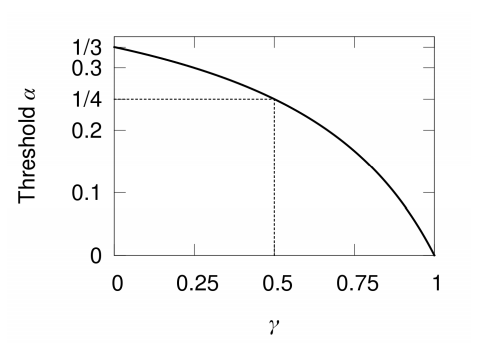
\includegraphics[width=130mm,scale=1]{tr.png}\\
\\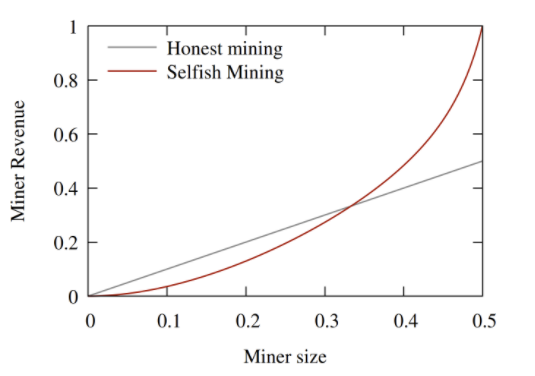
\includegraphics[width=130mm,scale=1]{mr.png}\\
\section{Consider the fact that most miners now join mining pools to mine
cryptocurrencies, what’s the economic consequence of the selfish mining
vulnerability?}
First, the longer the hidden selfish chain exist, the larger the computation power wasted.
New honest miners never gain revenues while their electricity cost increases from the beginning of mining.\\
Second, the significant revenue due to selfish mining attracts new selfish miners to join.
More selfish miners' joining causes the pure hashrate of longest chain to decrease 
even though more mining power joined. 
The value of cryptocurrencies will depreciate due to low hashrate of transaction completion.
\section{Search the web to survey the mining pool distributions of top cryptocurrencies:
BTC, ETH, LTC, XMR, and ZEC. How many of them are vulnerable to selfish mining
attacks?}
From the paper "On the Profitability of Selfish Mining Against
Multiple Difficulty Adjustment Algorithms",
All of them are more or less possible to fall into selfish mining attack.
But the possibility of profitability by selfish mining varies.
\begin{table}[h]
    \small
    \begin{threeparttable}
        \begin{tabular}{|p{4cm}|p{10cm}|}
        \hline
        \textbf{File} &	\textbf{Description} \\
        \hline
        BTC \& ETH \& LTC & Lower risk than described in 
        the literature due to  the lengthy period leading up to the difficulty
        adjustment.\\
        \hline
        XMR & Resistant to selfish mining due to miners' taking longer time 
        on difficulty adjustment
        for each block.\\
        \hline
        ZEC & The higher "MedianTimePast" provides 
        strong protection against selfish mining\\
        \hline
        \end{tabular}
    \end{threeparttable}
    \caption{Selfish mining risk}
    \label{table:smr}
\end{table}
\section{Describe the rationale of the block withholding attack. Why this can be a strategy
for a large mining pool to attack small mining pools.}
\section{In reality, selfish mining does not happen very often but the block withholding
attack happens a lot. What’s the reasons behind this?}
\end{document}